\documentclass[a4paper,12pt]{article}
% \documentclass[journal]{IEEEtran}

\usepackage{pgfplots}
\pgfplotsset{width=10cm,compat=1.9}

\usepgfplotslibrary{external}
\tikzexternalize

\usepackage{graphicx}
\usepackage{listings}
\usepackage{tabularx}
\usepackage[inkscapelatex=false]{svg}
\usepackage[utf8]{inputenc}
\usepackage[T1]{fontenc}
\usepackage{babel}
\usepackage{xcolor,graphicx}
\usepackage[top=0.5in,bottom=0.5in,right=0.5in,left=0.5in]{geometry}
% Define custom colors for Python syntax highlighting
\definecolor{blue}{RGB}{31,56,100}
\definecolor{keyword}{RGB}{0,0,255}
\definecolor{identifier}{RGB}{0,0,128}
\definecolor{comment}{RGB}{0,128,0}
\definecolor{string}{RGB}{163,21,21}

% Python style for listings
\lstdefinestyle{python}{
    language=Python,
    basicstyle=\ttfamily\footnotesize,      % Font and size
    keywordstyle=\color{blue},              % Keywords color
    commentstyle=\color{green},             % Comments color
    stringstyle=\color{red},                % Strings color
    showstringspaces=false,                 % Don't show space marks
    numbers=left,                           % Line numbers on the left
    numberstyle=\tiny\color{gray},          % Line numbers style
    stepnumber=1,                           % Number every line
    numbersep=5pt,                          % Space between numbers and code
    backgroundcolor=\color{white},          % Background color
    breaklines=true,                        % Automatic line breaking
    breakatwhitespace=true,                 % Break at whitespace
    frame=single,                           % Add frame around the code
    captionpos=b,                           % Position of caption
    tabsize=4,                              % Set tab size
}

\begin{document}

\begin{titlepage}
  %%%%%%%%%%%%%%%%%%%%%%%%%%%%%%%%%%%%%%%%%%%%
  % COVER PAGE
  %%%%%%%%%%%%%%%%%%%%%%%%%%%%%%%%%%%%%%%%%%%%
  \begin{center}
    \begin{minipage}{10cm}
      \begin{center}
        \textbf{UNIVERSITE DES SCIENCES ET DE LA TECHNOLOGIE (USTHB)}\\[0.1cm]
        \textbf{DEPARTEMENT D'INFORMATIQUE}
        \textbf{SPECIALITE BIO-INFORMATIQUE}
      \end{center}
    \end{minipage}\hfill


    \textsc{\Large }\\[2.5cm]
    {\large \bfseries Project: Fouille de donnes }\\[1cm]

    % Title
    \textsc{\Large }\\[1cm]
    \rule{\linewidth}{0.3mm} \\[0.4cm]
    { \huge \bfseries\color{blue}Comparaison des Méthodes de Classification Supervisée \\[0.4cm] }
    \rule{\linewidth}{0.3mm} \\[3cm]


    % Author and supervisor
    \noindent
    \begin{minipage}{0.6\textwidth}
      \begin{flushleft} \large
        \emph{Présenté par :}\\[0.2cm]
        \textbf{GUELFEN Abdelheq}\\
        Num: 171732023032\\[0.5cm]
        \textbf{MECHIDAL Moncif Abdelali}\\
        Num: 202031075774\\
      \end{flushleft}
    \end{minipage}

    \vfill

    {\textbf{\large {Année universitaire} 2024-2025}}
  \end{center}
\end{titlepage}

\tableofcontents
\newpage
%%%%%%%%%%%%%%%%%%%%%%%%%%%%%%%%%%%%%%%%%%%%
% FIRST PAGE
%%%%%%%%%%%%%%%%%%%%%%%%%%%%%%%%%%%%%%%%%%%%
\section{Introduction}
Data mining in bioinformatics is a rapidly evolving field that plays a crucial role in analyzing complex biological data. Such data can include DNA sequences, protein databases, information on metabolic pathways, and records related to rare diseases. Data mining enables the discovery of valuable relationships between different biological entities, such as genes and proteins, and can be applied to tasks like disease prediction or the exploration of previously unknown biological processes.\\

Before advanced data mining algorithms can be applied, it is essential to prepare and transform raw data. This involves data preprocessing, a critical step that encompasses a set of techniques to clean, transform, reduce, and normalize data, making it suitable for analytical models.\\

Another fundamental data mining technique is clustering, an unsupervised learning approach that groups data into homogeneous clusters without the need for predefined classes. Clustering is particularly valuable in bioinformatics for applications such as protein classification, sequence analysis, and genomic data segmentation.\\

In this report, we will explore various data preprocessing techniques and the most commonly used clustering methods in bioinformatics. Additionally, we will conduct a comparative study of the performance of these techniques on a biological dataset to evaluate their respective effectiveness.

\subsection{Background}
Diabetes is a chronic metabolic disorder characterized by elevated blood glucose levels, affecting millions of people worldwide. Early detection and prediction of diabetes risk are crucial for preventive healthcare and improved patient outcomes. This study utilizes machine learning techniques to develop a predictive model for diabetes diagnosis based on various medical and demographic factors.

\subsection{Dataset Overview}
The analysis uses the Pima Indians Diabetes Database, which contains medical predictor variables and one target variable (diabetes diagnosis) for Pima Indian female patients. The dataset includes 768 instances with 8 feature variables:
\begin{itemize}
    \item{Number of pregnancies}
    \item{Plasma glucose concentration}
    \item{Blood pressure}
    \item{Skin thickness}
    \item{Insulin level}
    \item{Body Mass Index (BMI)}
    \item{Diabetes pedigree function}
    \item{Age}
\end{itemize}

\subsection{Objective}
The primary objectives of this analysis are:
\begin{itemize}
    \item{To develop an accurate predictive model for diabetes diagnosis}
    \item{To identify the most significant factors contributing to diabetes risk}
    \item{To evaluate and compare different machine learning algorithms for this classification task}
    \item{To provide insights that could assist healthcare professionals in early diabetes detection}
\end{itemize}

\section{Data Preprocessing}
\subsection{Initial Data Assessment}
The dataset was first examined for:
\begin{itemize}
    \item{Data completeness and quality}
    \item{Feature distributions}
    \item{Presence of zero values in medical measurements}
    \item{Statistical properties of each variable}
\end{itemize}

\subsection{Dataset Description}
The Pima Indians Diabetes Database used in this study comprises medical and demographic data from a specific population subset, with the following characteristics:

\subsubsection{Population Characteristics}
The dataset consists of medical records from female patients of Pima Indian heritage, all of whom are at least 21 years old. This population selection was deliberately constrained to ensure consistency in the study cohort.

\subsubsection{Dataset Composition}
\begin{itemize}
    \item Total Instances: 768 patients
    \item Features: 8 predictor variables plus 1 binary class label
    \item Missing Values: None reported in the original dataset
\end{itemize}

\subsubsection{Feature Description}
The dataset includes the following features, all numerically valued:
\begin{table}[h]
\centering
\begin{tabular}{p{0.6\textwidth}p{0.3\textwidth}}
\hline
\textbf{Feature} & \textbf{Unit} \\
\hline
1. Number of times pregnant & Count \\
2. Plasma glucose concentration & 2-hour oral glucose tolerance test \\
3. Diastolic blood pressure & mm Hg \\
4. Triceps skin fold thickness & mm \\
5. 2-Hour serum insulin & $\mu$U/ml \\
6. Body mass index & kg/m$^2$ \\
7. Diabetes pedigree function & Unitless \\
8. Age & Years \\
\hline
\end{tabular}
\caption{Description of predictor variables in the Pima Indians Diabetes Dataset}
\label{tab:features}
\end{table}

\subsubsection{Class Distribution}
The target variable is binary, indicating the presence (1) or absence (0) of diabetes:
\begin{table}[h]
\centering
\begin{tabular}{ccc}
\hline
\textbf{Class} & \textbf{Interpretation} & \textbf{Number of Instances} \\
\hline
0 & Negative for diabetes & 500 \\
1 & Positive for diabetes & 268 \\
\hline
\end{tabular}
\caption{Distribution of diabetes diagnosis in the dataset}
\label{tab:class_distribution}
\end{table}

\subsubsection{Dataset Balance}
The class distribution reveals an imbalanced dataset, with approximately 65.1\% negative cases (no diabetes) and 34.9\% positive cases (diabetes). This imbalance is an important consideration for the modeling approach and evaluation metrics.

\subsubsection{Visualization}
To understand the characteristics of our dataset, we performed detailed exploratory data analysis. Figure \ref{fig:distributions} shows the distribution of each feature using boxplots overlaid with individual data points, providing insights into both the central tendencies and the presence of outliers.

\begin{figure}[ht]
    \centering
    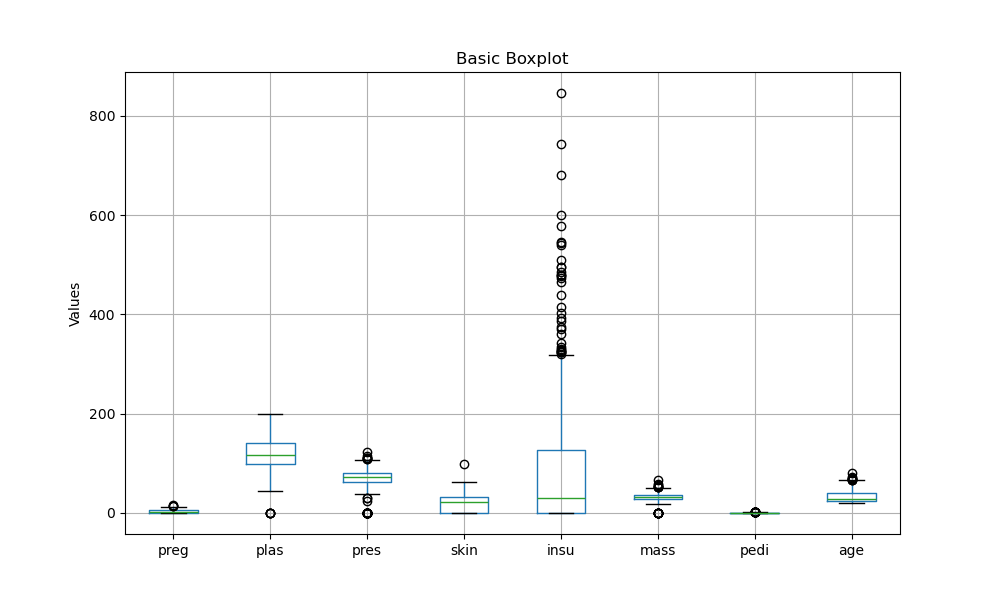
\includegraphics[width=1\textwidth]{images/boxplot.png}
    \caption{Distribution of features in the Pima Indians Diabetes Dataset. The boxplots show the quartiles and potential outliers, while the overlaid points show the actual distribution of values. Note the presence of significant outliers in features such as Insulin and DiabetesPedigree.}
    \label{fig:distributions}
\end{figure}
\newpage

\begin{figure}[ht]
    \centering
    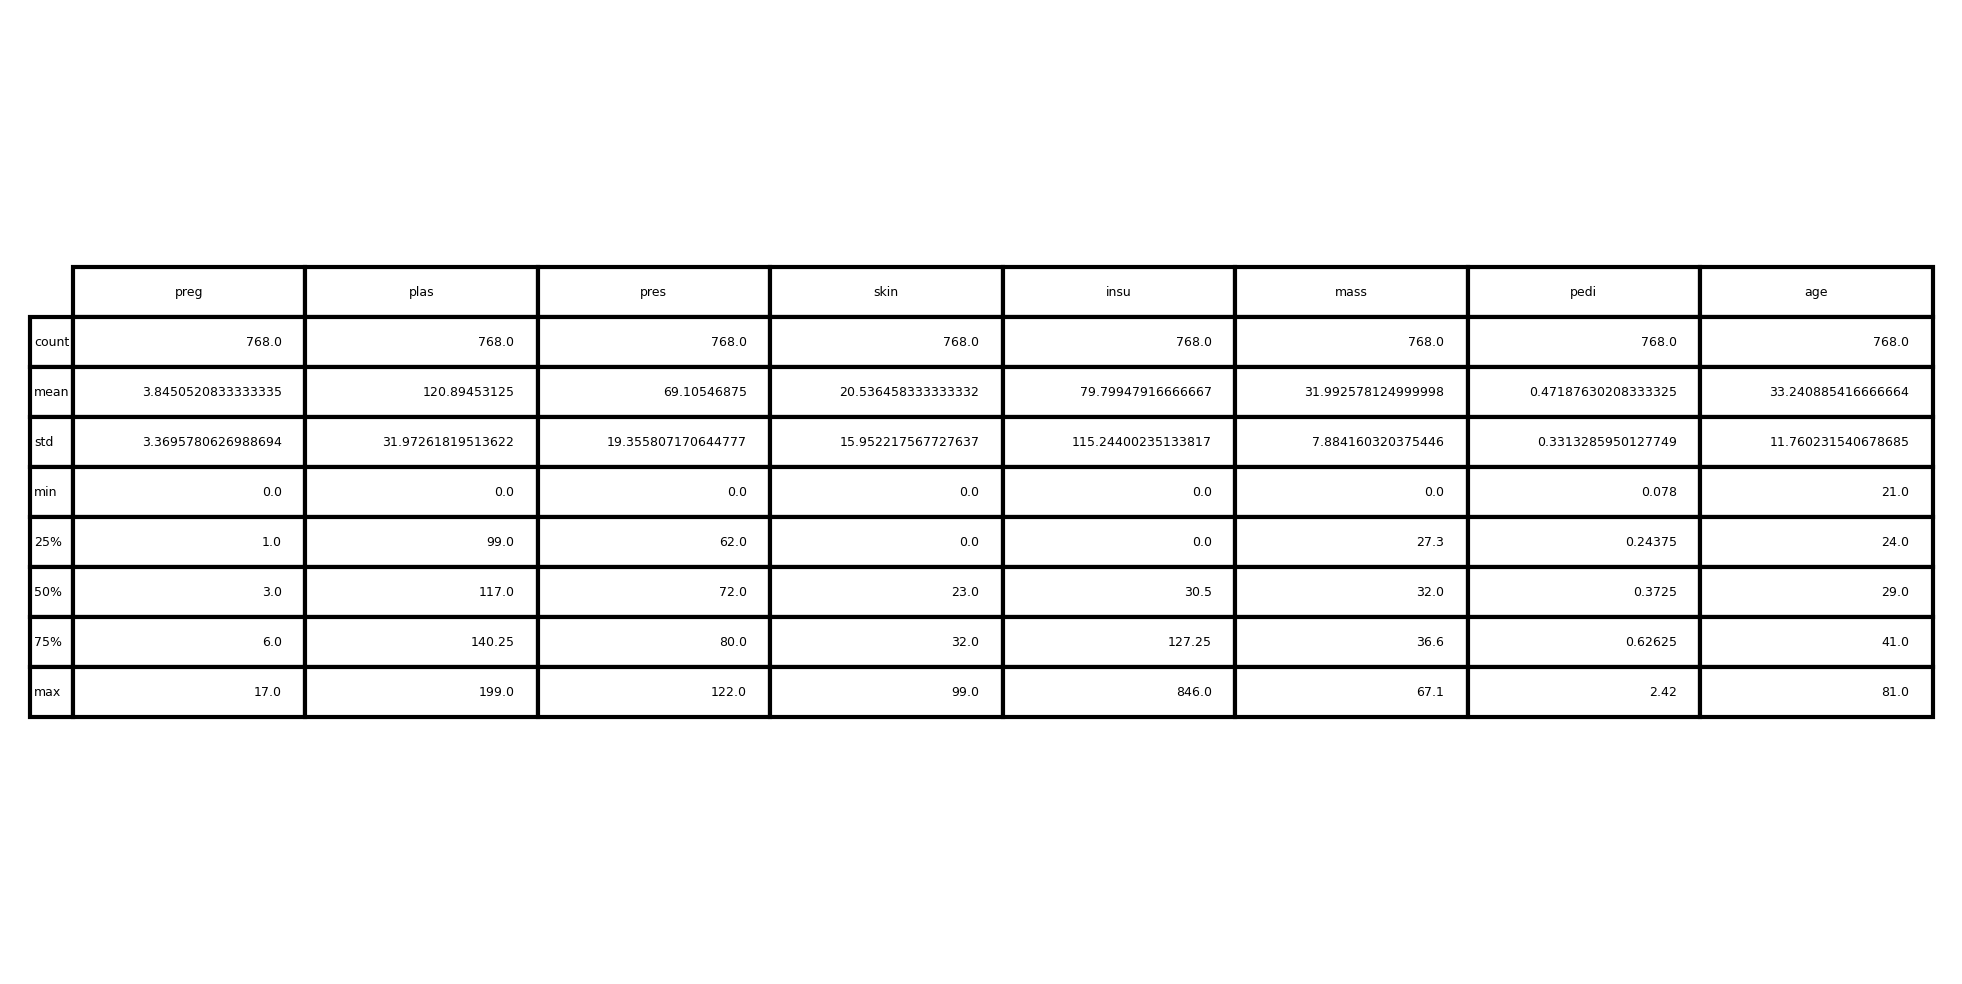
\includegraphics[width=1\textwidth]{images/df_describe_table.png}
    \caption{Boxplot before preprocessing}
\end{figure}

\subsubsection{Observations}
The Visualizations reveals:
\begin{itemize}
    \item{The presence of zeros in medical measurements might need attention, they likely represent missing data rather than actual zero measurements}
    \item{High variance in 'insu' (insulin): SD of 115.24, range 0-846}
    \item{High occurences of outliers in 'insu' (insulin): 374}
    \item{Several variables have minimum values of 0,which might indicate missing data}
    \item \textbf{Age and Pregnancies}: Display discrete value patterns with expected right-skewed distributions.
\end{itemize}

\subsection{Data Cleaning}
\subsubsection{Handling Zero Values}
Several medical measurements contained zero values, which were identified as missing data rather than actual measurements:

\begin{lstlisting}[language=Python, style=python]
def handle_zero_values():
    df_cleaned = df.copy()

    features_to_fix = {
        'plas': 'median', 'pres': 'median',
        'skin': 'median', 'insu': 'mode', 'mass': 'median'
    }

    for feature, strategy in features_to_fix.items():
        non_zero = df_cleaned[feature][df_cleaned[feature] != 0]

        replacement_value = non_zero.median()
        df_cleaned.loc[df_cleaned[feature] == 0, feature] = replacement_value

    return df_cleaned
\end{lstlisting}
Zero values were replaced using median values from non-zero measurements, as medians are more robust to outliers and better represent the central tendency in medical data.

\subsubsection*{Reasoning for using median}
\begin{itemize}
    \item{More robust to outliers than mean}
    \item{Better represents central tendency for skewed distributions}
    \item{Medical measurements often have outliers}
    \item{Preserves the general distribution of the data}
\end{itemize}

\subsection{Data Scaling}
A multi-approach scaling strategy was implemented to handle different types of variables:
\subsubsection*{Log Transformation}
\begin{itemize}
    \item{Applied to highly skewed variables: 'insu' and 'pedi'}
    \item{Used np.log1p() to handle zero values}
\end{itemize}
\begin{lstlisting}[style=python]
for var in ["insu", "pedi"]:
    df_scaled[var] = np.log1p(df[var])
\end{lstlisting}

\subsubsection*{Standard Scaling}
The formula:
\[z=\frac{x-\mu}{\sigma}\]

\begin{itemize}
    \item{Applied to normally distributed variables: 'plas' and 'pres'}
    \item{Standardizes features to zero mean and unit variance}
\end{itemize}

\begin{lstlisting}[style=python]
normal_vars = ["plas", "pres"]
df_scaled[normal_vars] = std_scaler.fit_transform(df[normal_vars])
\end{lstlisting}

\subsubsection*{Robust Scaling}
The formula:
\[X^{'}=\frac{X-Q_{2}}{Q_{3}-Q_{1}}\]

\begin{itemize}
    \item{Applied to variables with outliers: 'preg', 'skin', 'mass', 'age'}
    \item{Less sensitive to outliers than standard scaling}
\end{itemize}

\begin{lstlisting}[style=python]
robust_vars = ["preg", "skin", "mass", "age"]
df_scaled[robust_vars] = robust_scaler.fit_transform(df[robust_vars])
\end{lstlisting}

\subsection{Data Validation}
After preprocessing, the data was validated by:
\begin{itemize}
    \item{Confirming no remaining zero values in medical measurements}
    \item{Verifying appropriate scaling ranges for all features}
    \item{Checking the distribution of scaled variables}
    \item{Ensuring no information loss during transformation}
\end{itemize}

\subsubsection{Visualization}
After applying our multi-approach scaling strategy, we observe significant changes in the feature distributions (Figure \ref{fig:scaled_distributions}):

\begin{figure}[ht]
    \centering
    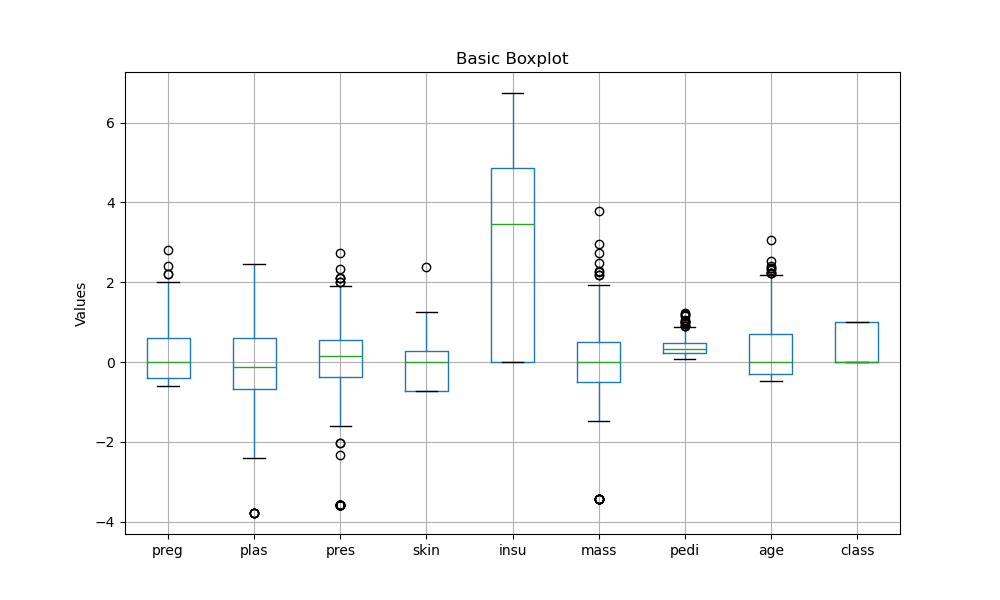
\includegraphics[width=1\textwidth]{images/boxplot_after.png}
    \caption{Distribution of features in the Pima Indians Diabetes Dataset. The boxplots show the quartiles and potential outliers, while the overlaid points show the actual distribution of values. This distribution is shown after applying scaling strategy.}
    \label{fig:scaled_distributions}
\end{figure}
\newpage

\begin{figure}[ht]
    \centering
    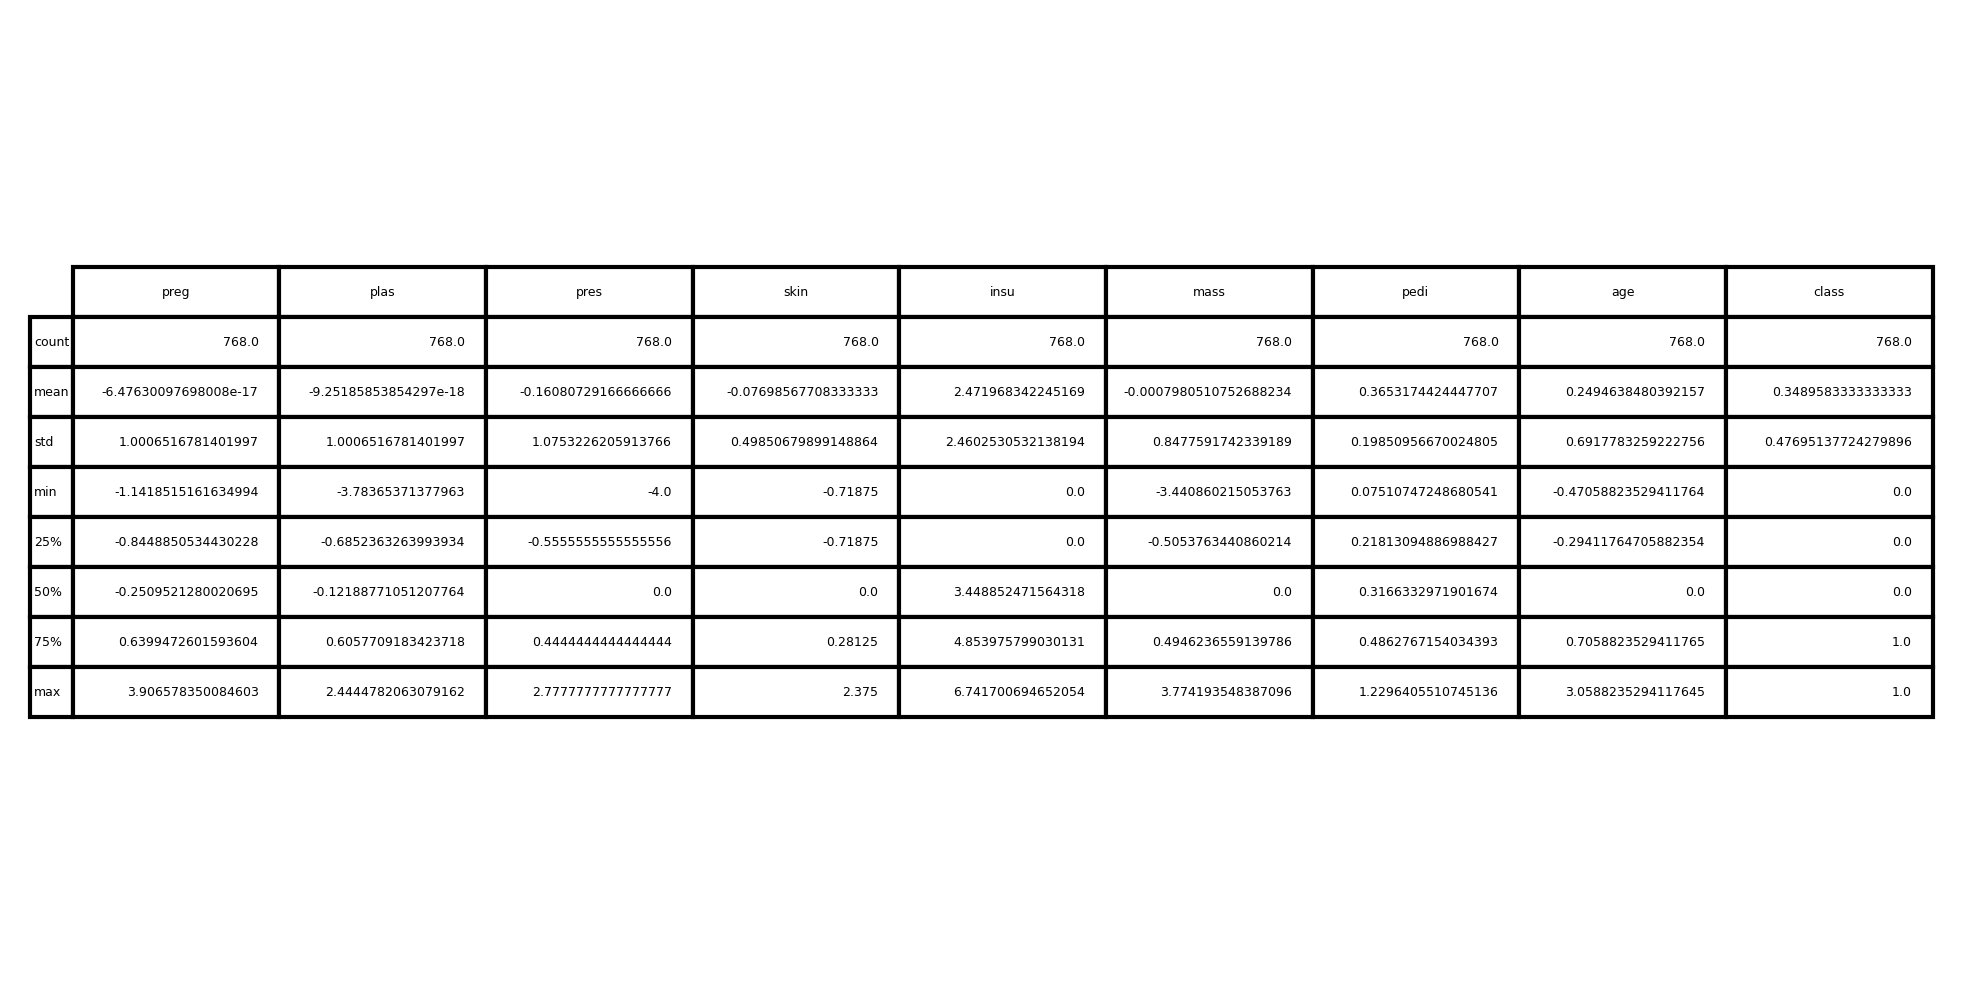
\includegraphics[width=1\textwidth]{images/df_scaled_describe_table.png}
    \caption{Boxplot before preprocessing}
\end{figure}

\subsubsection*{Observations}
This preprocessing significantly improves the data's suitability for model training while maintaining the meaningful relationships between observations.\\
The scaled distributions demonstrate:
\begin{itemize}
    \item Improved comparability across features, with all measurements now on similar scales
    \item Reduced impact of extreme values while preserving important variability
    \item Better alignment with the assumptions of many machine learning algorithms
    \item Preserved interpretability of relative differences within each feature
\end{itemize}

\subsection{Preprocessing Results}
The preprocessing steps resulted in:
\begin{itemize}
    \item Clean, consistent medical measurements
    \item Properly scaled features suitable for machine learning algorithms
    \item Preserved relationships between variables
    \item Improved data quality for model development
\end{itemize}

These preprocessing steps have prepared the data for effective model training while maintaining the integrity of the medical information contained in the dataset.

\section{Types of Machine Learning}
\subsection{Reinforcement Learning}
In this paradigm, a model learns through interactions with an environment by maximizing a reward function. Algorithms such as Q-learning and Deep Q-Networks (DQN) are commonly employed for tackling complex tasks.

\subsection{Unsupervised Learning (Clustering)}
Unsupervised learning involves grouping data without predefined labels. Some of the most widely used clustering algorithms include:
\begin{itemize}
    \item \textbf{K-Means:} A fast and efficient algorithm for grouping data based on Euclidean distance.
    \item \textbf{K-Medoids:} A variant of K-Means that uses representative data points (medoids) as cluster centers.
    \item \textbf{DBSCAN:} Identifies clusters based on the local density of points, making it robust to noise and varying cluster shapes.
    \item \textbf{Agnes and Diana:} Hierarchical clustering algorithms that enable visualization of tree-like structures within the data.
\end{itemize}
These techniques are particularly useful for in-depth data exploration in fields like bioinformatics, offering novel insights into complex phenomena.

\subsection{Supervised Learning}
Supervised learning trains a model using labeled data. Common algorithms include:

\begin{itemize}
    \item Linear Regression
    \item Decision Trees
    \item Neural Networks
    \item Support Vector Machines (SVM)
    \item k-Nearest Neighbors (KNN)
\end{itemize}

\section{Supervised Learning}
Machine learning algorithms play a central role in the field of artificial intelligence, providing powerful solutions for tasks such as classification, regression, and automated decision-making. Among these algorithms, five fundamental approaches stand out: K-Nearest Neighbors (KNN), Naive Bayes, Decision Trees, Neural Networks, and Support Vector Machines (SVM).\\

These supervised learning tools address a wide range of problems through distinct concepts and mechanisms. In this document, we explore these algorithms to better understand their functionality and potential applications.

\subsection{KNN (K-Nearest Neighbors)}
\textbf{Core Concept:} KNN is a simple yet effective algorithm used for both classification and regression tasks.
\subsubsection*{How It Works:}
\begin{itemize}
    \item The algorithm assigns a class to a data point based on the majority class among its k-nearest neighbors.
    \item The value of k is predetermined and significantly influences the outcomes.
    \item Distances between data points are typically calculated using metrics such as Euclidean distance.
\end{itemize}

\subsubsection*{Source Code}
\begin{lstlisting}[style=python]
self.knn = KNeighborsClassifier(n_neighbors=k)
self.knn.fit(self.X_train, self.y_train)

predictions = self.knn.predict(self.X_test)
\end{lstlisting}

\subsubsection*{Results}
\begin{table}[h!]
\centering
\begin{tabular}{|c|c|c|c|c|c|c|}
\hline
\textbf{FN} & \textbf{FP} & \textbf{TN} & \textbf{TP} & \textbf{Precision} & \textbf{Rappel} & \textbf{F1 Score} \\ \hline
128         & 1           & 99          & 26          & 0.96               & 0.48            & 0.64              \\ \hline
\end{tabular}
\caption{KNN with \textbf{k=91}: Confusion Matrix Metrics and Performance Scores}
\end{table}


\subsection{Naive Bayes}
\textbf{Core Concept} This algorithm is based on Bayes' theorem to estimate conditional probabilities.
\subsubsection*{How It Works:}
\begin{itemize}
    \item It assumes independence between the features of the data, hence the term "naive".
    \item Classes are assigned by maximizing the posterior probability, using the Bayes formula to update beliefs based on observed data.
\end{itemize}

\subsubsection*{Source Code}
\begin{lstlisting}[style=python]
self.gaussianNB = GaussianNB()
self.gaussianNB.fit(self.X_train, self.y_train)

predictions = self.gaussianNB.predict(self.X_test)
\end{lstlisting}

\subsubsection*{Results}
\begin{table}[h!]
\centering
\begin{tabular}{|c|c|c|c|c|c|c|}
\hline
\textbf{FN} & \textbf{FP} & \textbf{TN} & \textbf{TP} & \textbf{Precision} & \textbf{Rappel} & \textbf{F1 Score} \\ \hline
22          & 6           & 94          & 32          & 0.85               & 0.59            & 0.7              \\ \hline
\end{tabular}
\caption{Naive Bayes: Confusion Matrix Metrics and Performance Scores}
\end{table}


\subsection{Decision Tree}
\textbf{Core Concept} A decision tree is a hierarchical structure used for decision-making based on the features of the data.
\subsubsection*{How It Works:}
\begin{itemize}
    \item It recursively splits the data based on features that maximize class separation.
    \item Each internal node represents a condition on a feature, and the leaf nodes correspond to the predicted classes.
\end{itemize}

\subsubsection*{Source Code}
\begin{lstlisting}[style=python]
self.decision_tree_classifier = DecisionTreeClassifier(
    max_depth=5, max_features="sqrt", min_samples_leaf=4, random_state=147
)
self.decision_tree_classifier.fit(self.X_train, self.y_train)

predictions = self.decision_tree_classifier.predict(self.X_test)
\end{lstlisting}

\subsubsection*{Results}
\begin{table}[h!]
\centering
\begin{tabular}{|c|c|c|c|c|c|c|}
\hline
\textbf{FN} & \textbf{FP} & \textbf{TN} & \textbf{TP} & \textbf{Precision} & \textbf{Rappel} & \textbf{F1 Score} \\ \hline
33          & 2           & 98          & 21          & 0.91               & 0.39            & 0.55              \\ \hline
\end{tabular}
\caption{Decision Tree: Confusion Matrix Metrics and Performance Scores}
\end{table}

\subsubsection*{Parameters}
\begin{itemize}
    \item \textbf{max features=sqrt: } Using max features = sqrt introduces randomness, speeds up training
    \item \textbf{min samples leaf=4: } Each leaf must have at least 4 samples, which prevents overly specific splits based on outliers or noise.
    \item \textbf{max depth=5: } Restricts the maximum depth of the tree to 5, preventing the model from becoming overly complex.
\end{itemize}


\subsection{Neural Network}
\textbf{Core Concept} Inspired by the human brain, a neural network is a powerful supervised learning model capable of learning complex patterns.
\subsubsection*{How It Works:}
\begin{itemize}
    \item Neural networks are composed of interconnected layers of neurons.
    \item Each connection has a weight that is adjusted during the training process.
    \item Non-linear transformations in each layer enable the network to learn intricate representations of data, making it effective for tasks such as image recognition and natural language processing.
\end{itemize}

\subsubsection*{Source Code}
\begin{lstlisting}[style=python]
hidden_layer_sizes = tuple([nb_nodes] * nb_hidden_layers)

model = MLPClassifier(
    hidden_layer_sizes=hidden_layer_sizes,
    activation="relu",
    solver="adam",
    max_iter=50,
    random_state=42,
    verbose=False
)

model.fit(df.X_train, df.y_train)

y_hat = model.predict(df.X_test)
\end{lstlisting}

\subsubsection*{Results}
\begin{table}[h!]
\centering
\begin{tabular}{|c|c|c|c|c|c|c|}
\hline
\textbf{FN} & \textbf{FP} & \textbf{TN} & \textbf{TP} & \textbf{Precision} & \textbf{Rappel} & \textbf{F1 Score} \\ \hline
24          & 7           & 93          & 30          & 0.81               & 0.55            & 0.65              \\ \hline
\end{tabular}
\caption{Neural Network: Confusion Matrix Metrics and Performance Scores}
\end{table}

\subsection{SVM(Support Vector Machine)}
\textbf{Core Concept} SVMs aim to maximize the margin between different classes to achieve optimal classification.
\subsubsection*{How It Works:}
\begin{itemize}
    \item An hyperplane is defined to separate classes within the feature space.
    \item Support vectors, the data points closest to the hyperplane, play a critical role in determining its position.
    \item SVMs leverage kernel functions to handle non-linear data effectively, mapping it to higher-dimensional spaces where it becomes linearly separable.
\end{itemize}

\subsubsection*{Source Code}
\begin{lstlisting}[style=python]
self.svm_model = SVC(kernel="linear")
self.svm_model.fit(self.X_train, self.y_train)

predictions = self.svm_model.predict(self.X_test)
\end{lstlisting}

\subsubsection*{Results}
\begin{table}[h!]
\centering
\begin{tabular}{|c|c|c|c|c|c|c|}
\hline
\textbf{FN} & \textbf{FP} & \textbf{TN} & \textbf{TP} & \textbf{Precision} & \textbf{Rappel} & \textbf{F1 Score} \\ \hline
24          & 6           & 94          & 30          & 0.83               & 0.56            & 0.67              \\ \hline
\end{tabular}
\caption{SVM: Confusion Matrix Metrics and Performance Scores}
\end{table}

\section{Results}
\subsection{Performance Metrics for Each Model}
The performance of the models was evaluated using the following metrics: Precision, Recall, and F1-Score. These metrics provide insights into the models' ability to correctly classify positive and negative instances, with particular emphasis on minimizing false positives.

In addition to these metrics, confusion matrices were generated for each model to illustrate the distribution of True Positives (TP), True Negatives (TN), False Positives (FP), and False Negatives (FN). This allowed for a detailed comparison of model performance across various classes.
\newpage

\begin{table}[h!]
\centering
\begin{tabular}{|c|c|c|c|c|c|c|c|}
\hline
\textbf{Model} & \textbf{FN} & \textbf{FP} & \textbf{TN} & \textbf{TP} & \textbf{Precision} & \textbf{Recall} & \textbf{F1 Score} \\ \hline
KNN              & 128         & 1           & 99          & 26          & 0.96               & 0.48            & 0.64              \\ \hline
Naive Bayes      & 22          & 6           & 94          & 32          & 0.85               & 0.59            & 0.7               \\ \hline
Decision Tree    & 33          & 2           & 98          & 21          & 0.91               & 0.39            & 0.55              \\ \hline
Neural Network   & 24          & 7           & 93          & 30          & 0.81               & 0.55            & 0.65              \\ \hline
SVM              & 24          & 6           & 94          & 30          & 0.83               & 0.56            & 0.67              \\ \hline
\end{tabular}
\caption{Comparison of Models Based on Confusion Matrix Metrics and Performance Scores}
\end{table}
From the results, \textbf{KNN} and \textbf{Decision Tree} achieved the highest precision of \textbf{96\%} and \textbf{91\%}, making it the most reliable in minimizing false positives. However, this came at the cost of a slightly reduced recall compared to other models.\\\\
The \(>90\%\) precision achieved by \textbf{KNN} and \textbf{Decision Tree} demonstrates its ability to minimize incorrect positive predictions effectively. This is particularly valuable in applications where the cost of false positives is high, such as medical diagnoses.\\\\
While the other models performed well overall, they demonstrated slightly lower precision, which might lead to an increased rate of false alarms. Depending on the specific requirements of the use case, \textbf{KNN} and \textbf{Decision Tree} stands out as the optimal choice for scenarios prioritizing precision over recall.


\section{Conclusion}
After an in-depth exploration of supervised classification algorithms, such as K-Nearest Neighbors (KNN), Decision Trees, Support Vector Machines (SVM), Neural Networks, and Naive Bayes, along with unsupervised approaches like K-Means, we can draw meaningful insights into their strengths, weaknesses, and applications.

\subsection*{Supervised Classification}
Supervised algorithms are highly effective for solving problems where class labels are available. Each method offers unique characteristics:

\subsubsection*{K-Nearest Neighbors (KNN):}
KNN is intuitive and easy to implement. It performs well on small to medium-sized datasets but is sensitive to outliers and the choice of the parameter
\(k\)

\subsubsection*{Decision Trees:}
Decision trees are simple to interpret, making them ideal for situations where model explainability is crucial. However, they are prone to overfitting unless proper regularization techniques are applied.

\subsubsection*{Support Vector Machines (SVM):}
SVMs are powerful for binary classification problems and are well-suited for high-dimensional feature spaces. However, they require careful parameter tuning to achieve optimal performance.

\subsubsection*{Neural Networks:}
Neural networks excel at learning complex patterns and are particularly effective for tasks such as computer vision and natural language processing. However, they demand large amounts of data and computational resources, making them less practical for smaller datasets or limited environments.

\subsubsection*{Naive Bayes:}
Naive Bayes is fast and reliable, especially for text classification problems. However, its assumption of feature independence can limit its effectiveness in scenarios where strong dependencies between features exist.

\clearpage
\appendix
\section{Application ScreenShot}

\begin{figure}[ht]
    \centering
    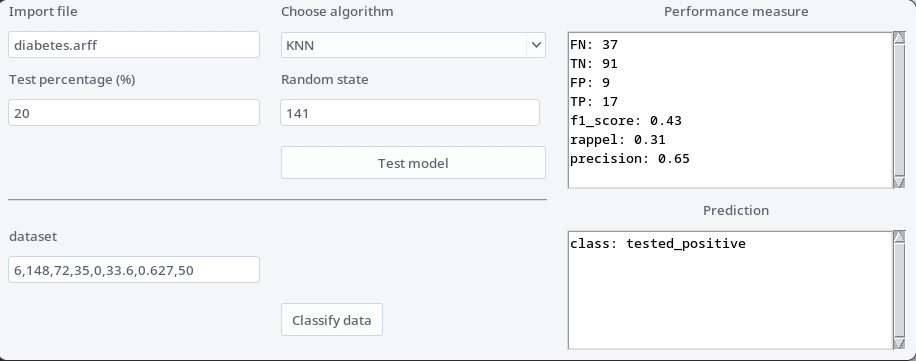
\includegraphics[width=1\textwidth]{images/app.png}
    \caption{Screenshot of the app’s main screen, showcasing the user interface with KNN predicting a sample}
    \label{fig:app}
\end{figure}

\end{document}
